\section{Presentation Logic Layer}

Our Web application is mainly developed in eight pages; not all of them are accessible by all users, it depends on their tier (see \ref{fig:users_tiers}). Also page functionalities depend on tier, i.e. when searching for an event, tier 1 users can see only events for tier 1 or lower, tier 2 users can see events for tier 2 or lower, and so on. More restrictions are made to users that haven't confirmed their mail yet.\\
Here above most important pages are listed, some are missing, s.e. login, signup pages, or the form to complete the registration.

\begin{itemize}
    \item \texttt{Home}: it's the landing page, when a user is logged it shows a list of events and a search bar. Otherwise, it shows the login page. It's accessible to all users.
    \item \texttt{Profile}: it shows the user's profile info and allows them to change them. It's accessible to all users.
    \item \texttt{My events}: it shows a list of events the user is participating in. It's accessible to all users.
    \item \texttt{Logout}: it allows to logout. It's accessible to all users.
    \item \texttt{(Admin) Create Event}: it allows one to create a new event and eventually change some information about them. It's accessible by tier 2 or above users.
    \item \texttt{(Admin) Search User}: it allows one to search for a user and eventually modify his profile. It's accessible by administrators.
    \item \texttt{(Admin) Create cause}: it allows one to create a new cause. It's accessible by administrators.
    \item \texttt{(Admin) Search cause}: it allows one to search for a cause and eventually modify or delete it. It's accessible by administrators.
\end{itemize}

\subsection{Signup page}
\begin{figure}[H]
    \centering
    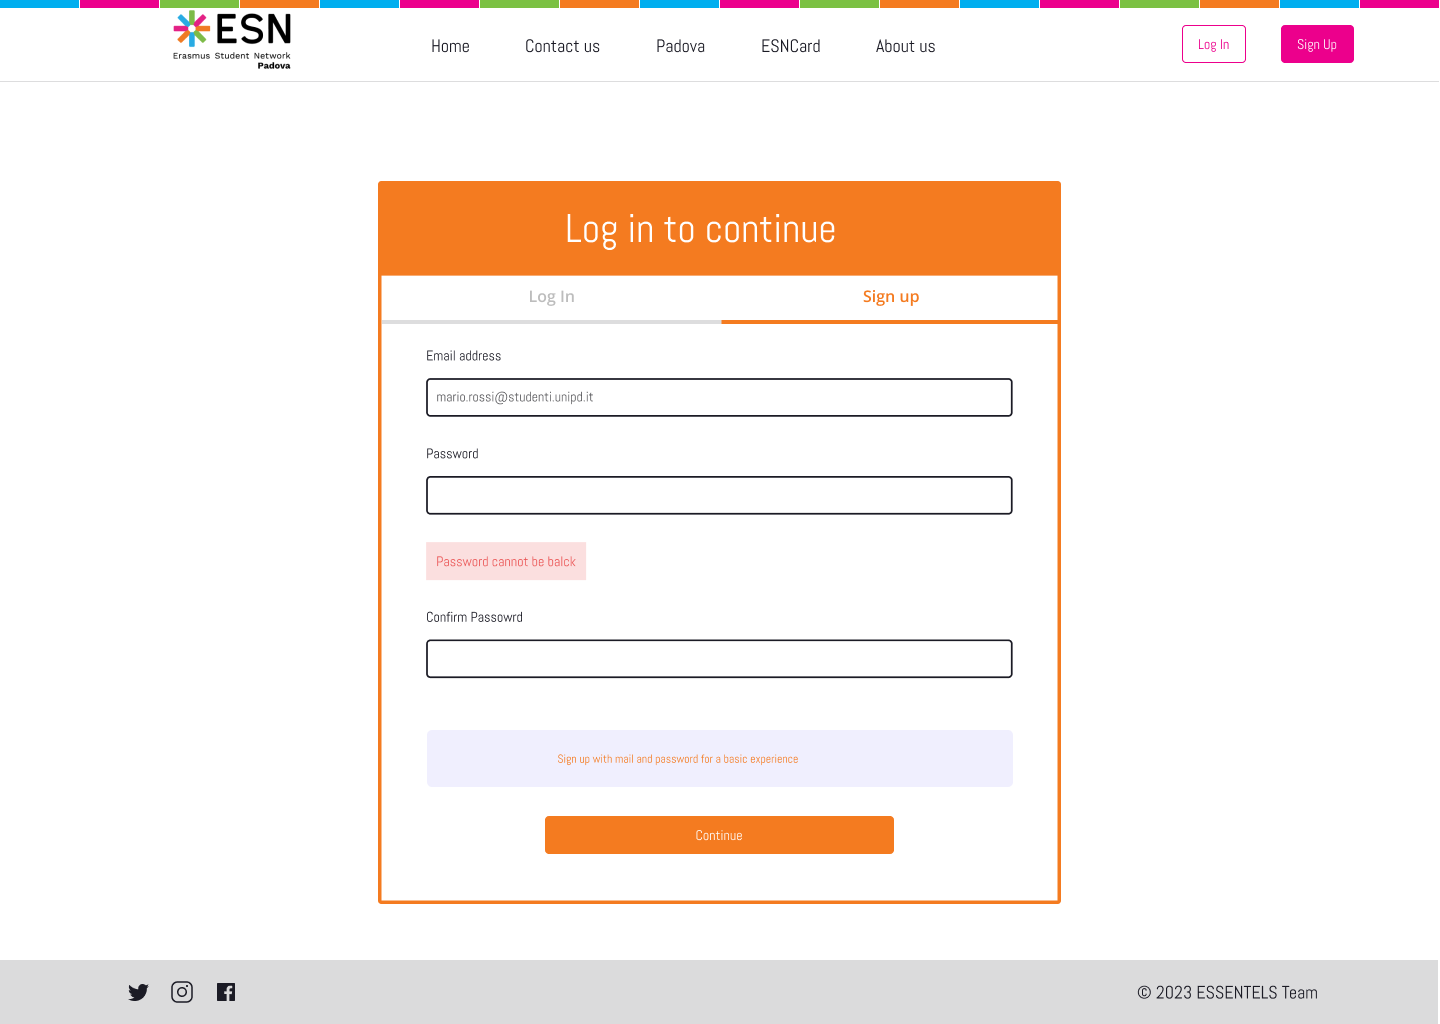
\includegraphics[width=0.5\textwidth]{images/signup.png}
    \caption{Sign up page}
    \label{fig:signup page}
\end{figure}
Users can sign up just with their mail and password. They will not have access only to their
0 events. For a better experience and more opportunities,
they are asked to complete their profile with a more detailed form, including those from
their hometown. This form is shown in \ref{fig:form} and described in next section.
\subsection{Registration form}
\begin{figure}[H]
    \centering
    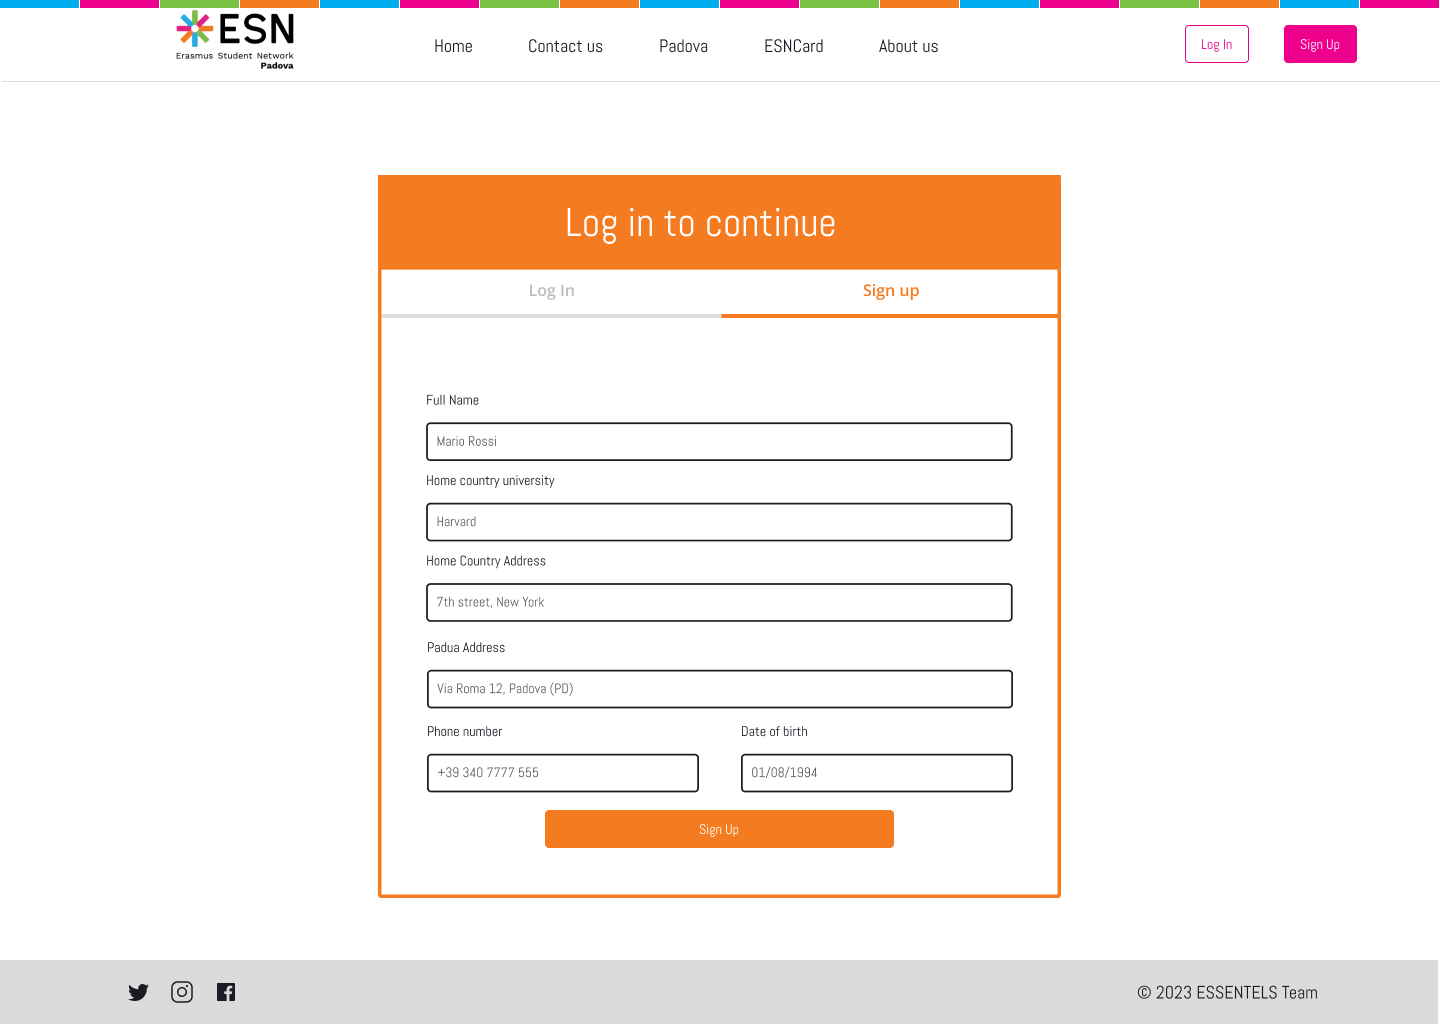
\includegraphics[width=0.5\textwidth]{images/form.png}
    \caption{Form for the full registration}
    \label{fig:form}
\end{figure}
When user wants to upgrade to tier 1 they have to pay their subscription (as shown in \ref{fig:payment}).
The form for a full profile asks for any information, here just a few are displayed, but the 
real form will have more than 10 input boxes. 
\subsection{Payment page}
\begin{figure}[H]
    \centering
    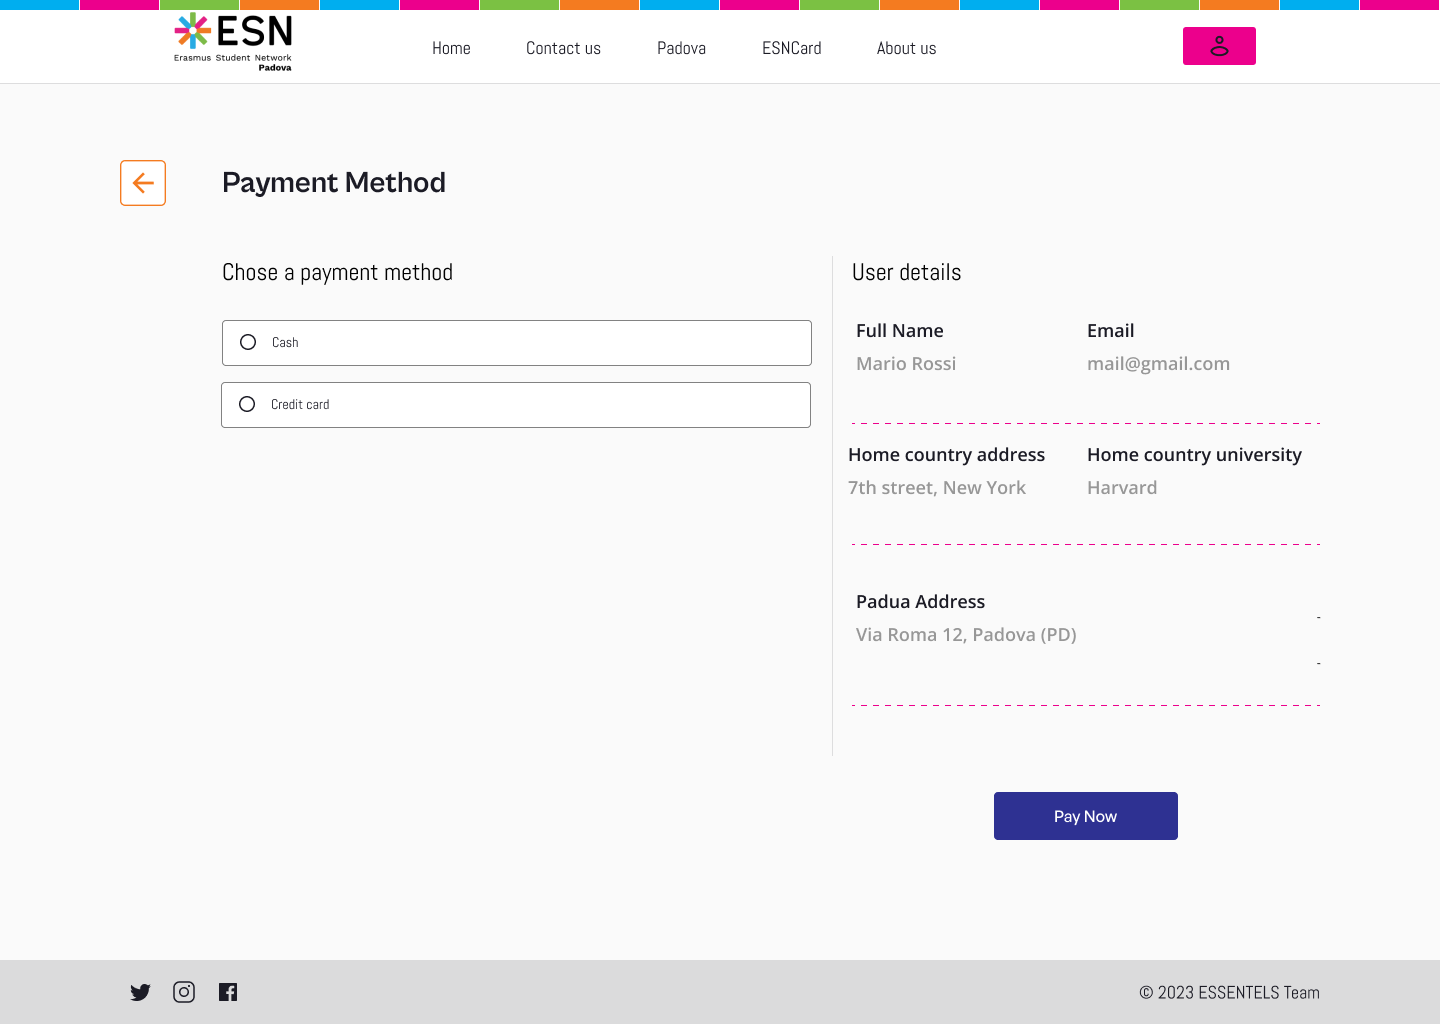
\includegraphics[width=0.5\textwidth]{images/PaymentMethod.png}
    \caption{Payment page}
    \label{fig:payment}
\end{figure}
When a user pays his subscription, he will become a tier 1 user. He will be able to participate in more
events. Still, he cannot create an event (only tier 3 or above users can do that). 
\subsection{Events list page}
\begin{figure}[H]
    \centering
    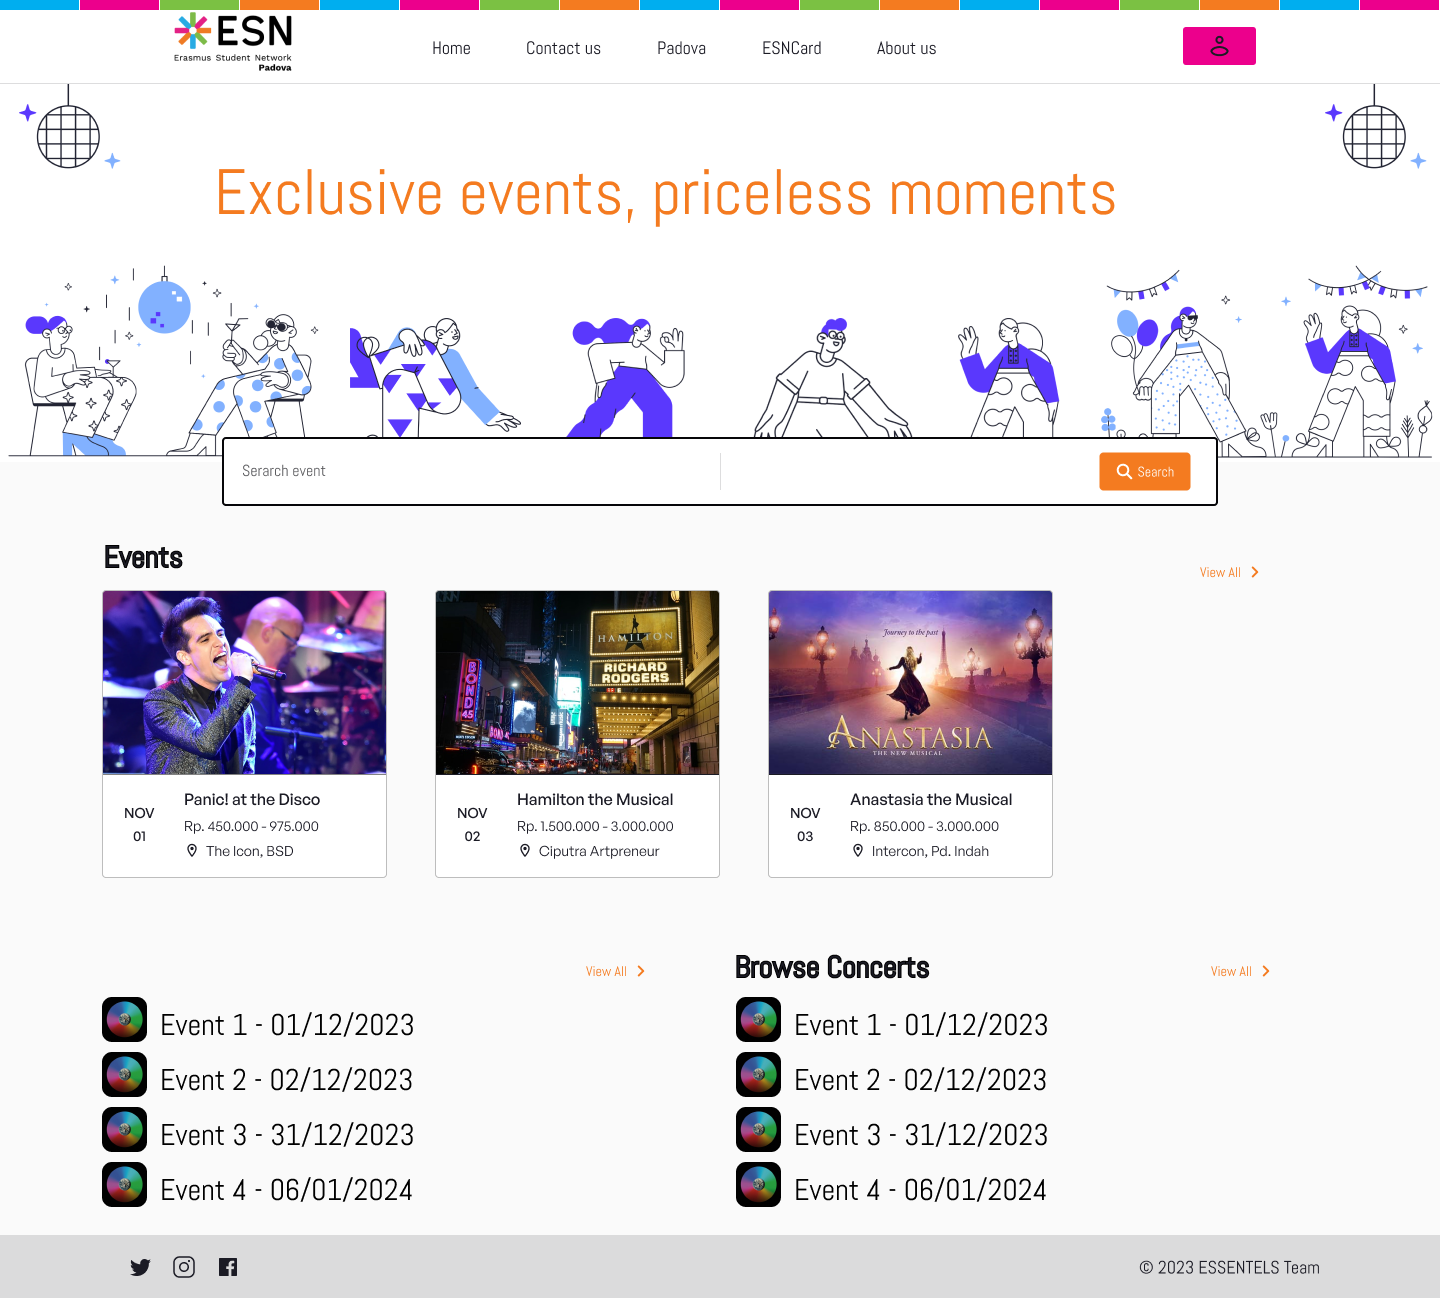
\includegraphics[width=0.5\textwidth]{images/EventList.png}
    \caption{Sign up page}
    \label{fig:events}
\end{figure}
Here all events are listed or filtered by tag or cause. Users are allowed to see only events for their tier
or lower ones. Since all events have a location, we decided -according to ESN volunteers- to keep
events automatically filtered by tier.\\
Searching by tag or by cause is actually made by a REST API: using GET, events are listed, and an administrator
can also use DELETE to delete an event. With a POST request, a new event can be created.\\
\subsection{Join event page}
\begin{figure}[H]
    \centering
    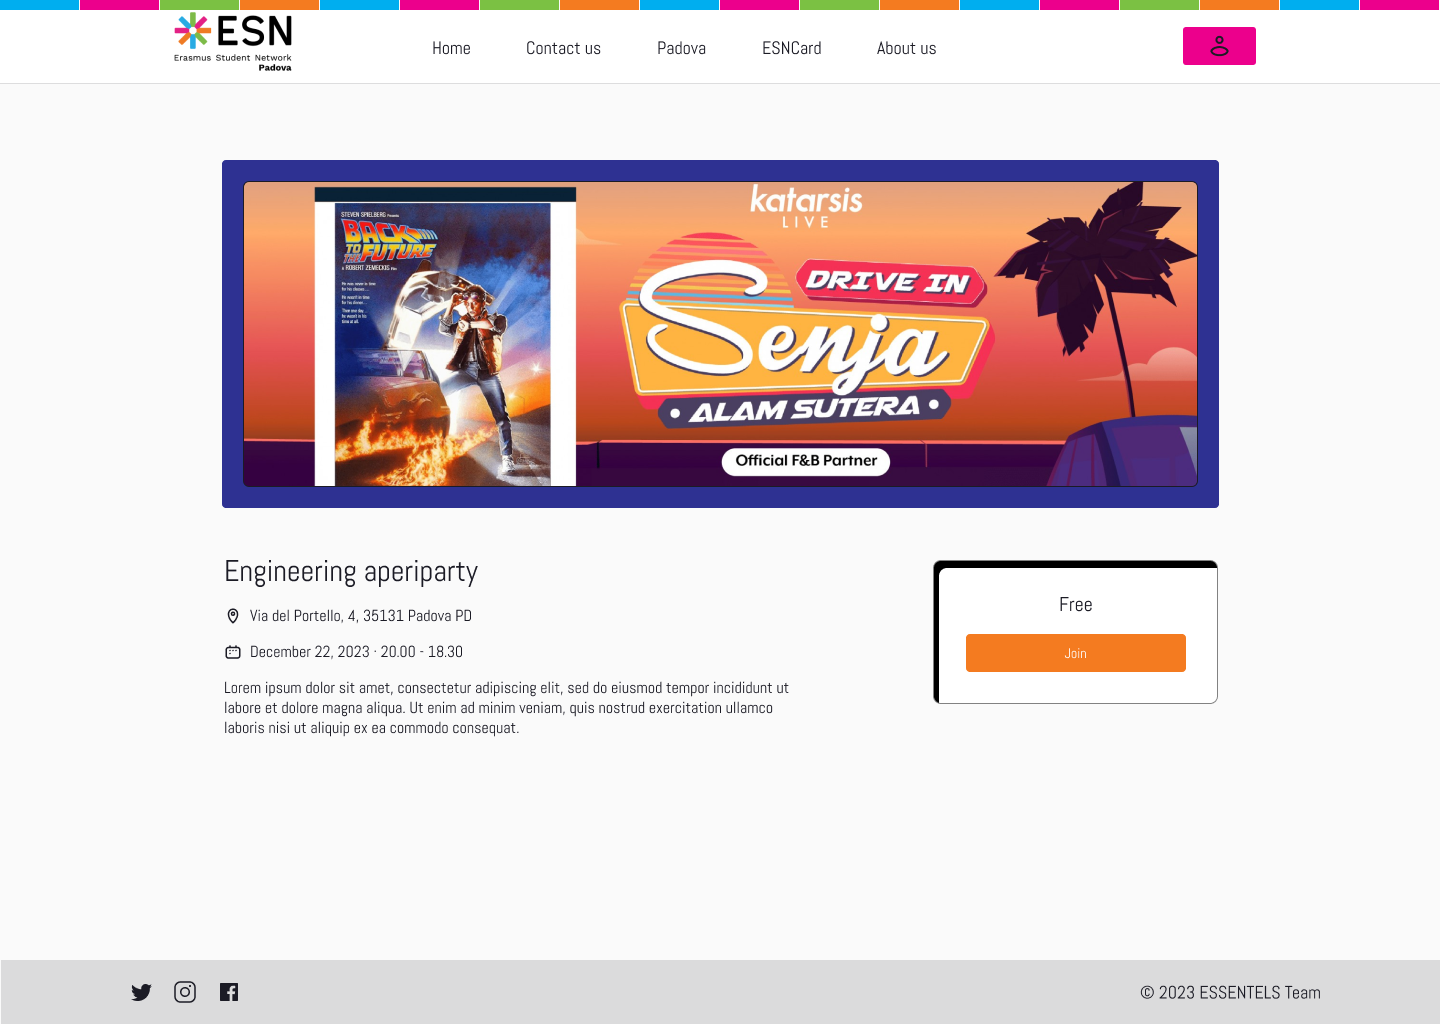
\includegraphics[width=0.5\textwidth]{images/JoinEvent.png}
    \caption{Sign up page}
    \label{fig:joinEvent}
\end{figure}
When a user wants to join an event, he can see all the details and the list of participants. Here
he can also see more detailed info about the event and confirm his participation. In case some events
will ask for a ticket one day, this page will redirect to a payment page, similar to \ref{fig:payment},
but linked to tickets for cinemas, parties etc.
\subsection{Change user info}
\begin{figure}[H]
    \centering
    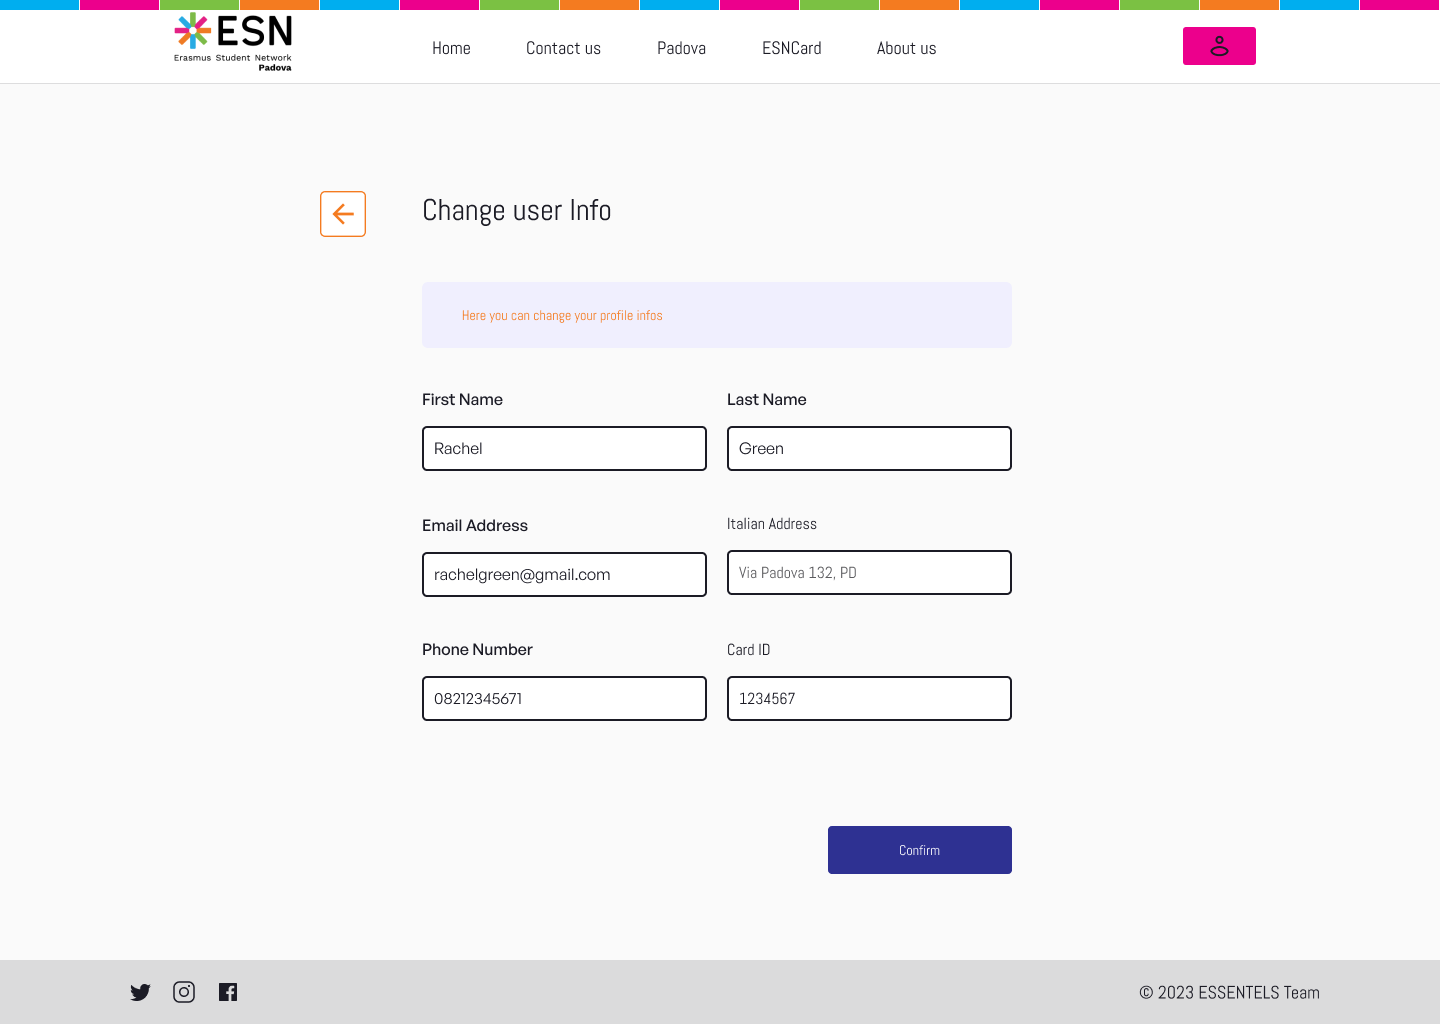
\includegraphics[width=0.5\textwidth]{images/ChangeUserDetail.png}
    \caption{Change user's info}
    \label{fig:change info}
\end{figure}
Users can change their profile info. This page can be accessed by each user for his own profile or 
by an admin for any user.